In section (\ref{sec:1_1_motivation}) we introduced boundary integral equations (\ref{eq:generic_int_equation:sec:1_1}) and their matrix representation (\ref{eq:linear_system:sec:1_1}), noting that it could alternatively be represented using hierarchical matrices. As we have seen, these matrix representations (HSS, $\mathcal{H}^2$ etc.) allow us to rapidly \textit{apply} the system matrix (\ref{eq:linear_system:sec:1_1}) with linear or near linear time complexity. In combination with modern \textit{iterative} methods, such as GMRES \cite{saad1986gmres}, with $O(n_k)$ iterations such that $n_k \ll N$ where $N$ is the number of unknowns in the system, the solution of such problems is brought into practical reach. However, there are situations in which iterative methods fall short. For example for problems which have \textit{multiple} right hand sides we wish to solve for. In such cases, recently developed \textit{fast direct} methods offer a promising alternative. The inversion of a dense linear system by classical direct methods, such as Gaussian Elimination or LU decomposition, have a complexity of $O(N^3)$. Fast direct methods however take advantage of the low-rank structure implicit in the matrix of (\ref{eq:generic_int_equation:sec:1_1}) to find an approximation for the inverse in a similar manner to the FMM. The main trade-off between fast direct methods and the iterative alternative is the relatively greater memory cost in having to pre-compute and store the matrix factorization.

Numerous approaches have been implemented for fast direct solvers for the matrix factorisations described in section (\ref{sec:1_1_motivation}). Here we introduce the `Recursive Strong Skeletonisation' (RS-S) algorithm of Minden et. al \cite{minden2017recursive}, which incorporates strong admissibility and has good properties for parallelisation. Our main contribution is the extension of this technique to effectively handle acoustic scattering problems at low to moderate frequencies where the size of the problem domain is less than a few hundred times the wavelength, building on the exterior Dirichlet case first presented in \cite{sushnikova2022fmm}. 

\subsection*{Problem Formulation}

We start by deriving the boundary integral equation for the boundary value problem described by the Helmholtz equation and an exterior Dirichlet boundary condition,

\begin{flalign}
    \label{eq:sec_3_1:helmholtz_ext_dir}
    (\Delta + k^2) u = 0, \> \> \text{in } \mathbb{R^d} \setminus \Omega \\
    u = f, \> \> \text{on } \Gamma \\ 
    \lim_{r \rightarrow \infty} r \left ( \frac{\partial u}{ \partial r} - iku \right ) = 0
\end{flalign}

The final line above describes a `radiation condition', which is required to maintain the uniqueness of $u$. Physically, the solution $u$ corresponds to the spatial distribution of a wave scattered from an object with domain $\Omega$ and boundary $\Gamma$ embedded in $\mathbb{R}^d$ where without loss of generality we will take $d=3$. 

Using the definition of the free space Green's function,

\begin{flalign}
    \Phi(\mathbf{x}, \mathbf{y}) = \frac{e^{ik|\mathbf{x} -\mathbf{y}|}}{4\pi |\mathbf{x} - \mathbf{y}|}
\end{flalign}

And defining,

\begin{flalign}
    K(\mathbf{x}, \mathbf{y}) = (\mathbf{n}(y) \cdot \nabla_{\mathbf{y}}\Phi(\mathbf{y}, \mathbf{x})) -ik \Phi(\mathbf{x}, \mathbf{y}) 
\end{flalign}

where $n(\mathbf{y})$ is the outwardly facing unit normal at $y \in \partial \Gamma$, we define the \textit{combined field representation} of $u$ as,

\begin{flalign}
    \label{eq:sec_3_1:combined_field_representation}
    u &= \int_\Gamma K(\mathbf{x}, \mathbf{y}) \sigma(\mathbf{y}) da(\mathbf{y}), \> \> \mathbf{x} \in \mathbb{R}^3 \setminus \Omega \\
    &= \int_\Gamma (\mathbf{n}(y) \cdot \nabla_{\mathbf{y}}\Phi(\mathbf{y}, \mathbf{x})) -ik \Phi(\mathbf{x}, \mathbf{y}) \sigma(\mathbf{y}) da(\mathbf{y}) \\
    &= (\mathcal{D} - ik \mathcal{S}) \sigma
\end{flalign}

where we also define the double layer, $\mathcal{D}$, and single layer, $\mathcal{S}$ potential operators. Representing $u$ in terms of layer potentials gives us a solution of the the PDE (\ref{eq:sec_3_1:helmholtz_ext_dir}), however the `surface density' $\sigma$ is unknown. Armed with a representation we can proceed to form a \textit{boundary integral equation} defined only along $\Gamma$ in terms of the the unknown $\sigma$,

\begin{flalign*}
    (\mathcal{D} -ik \mathcal{S} + \frac{1}{2})\sigma(\mathbf{x}) = f(\mathbf{x}), \> \> \mathbf{x} \in \Gamma
\end{flalign*}

Here we have used the well known \textit{jump relations} which describe a discontinuity in the value of the double layer potential operator as we approach the boundary. Further information about layer potentials, the particular benefits of the combined field representation and the jump relations can be found in appendix \ref{app:a_5:bie} For our purposes it's sufficient to recognise that this boundary integral equation motivates our work on fast direct solvers. Writing it in another form,

\begin{flalign}
    \frac{1}{2} \sigma(\mathbf{x}) + \int_\Gamma K(\mathbf{x}, \mathbf{y}) \sigma(\mathbf{y}) da(\mathbf{y}) = f(\mathbf{x})
\end{flalign}

we see that it can be discretised using a suitable method, such as the Galerkin or Nyström methods. Using Nyström we arrive at the following linear system,

\begin{flalign}
    \label{eq:sec_3_1:bie}
    \frac{1}{2} \sigma_i + \sum_{j=1, j \neq i}^N K(\mathbf{x}_i, \mathbf{x}_j) \sigma_j w_{ij} = f(x_i)
\end{flalign}

where $\mathbf{x}_i$ and $w_{ij}$ are the quadrature nodes and weights, respectively, and $\sigma_i$ is the approximation to $\sigma(\mathbf{x}_i)$. Solving this equation for $\sigma$, allows one to find the approximation of the general solution of the scattering problem (\ref{eq:sec_3_1:helmholtz_ext_dir}) in the exterior using (\ref{eq:sec_3_1:combined_field_representation}).

\subsection*{Recursive Strong Skeletonisation}

Consider a domain containing the discretisation points of the boundary $\Gamma$, $\mathbf{x}_i \in \Gamma$. We proceed to discretise with an adaptive, 2:1 balanced, octree. The idea of strong skeletonisation is then to use the \textit{interpolative decomposition} (ID) \cite{cheng2005compression}, a dense matrix compression algorithm, to globally compress matrices with low-rank structure for the case in which only particular off-diagonal blocks are low-rank. In our problem of interest, (\ref{eq:sec_3_1:bie}), where the low-rank assumption only applies when two nodes of an octree are strongly admissible with respect to each other, i.e. the far-field interactions via the kernel of the integral equation.

\begin{definition}[Interpolative Decomposition (ID)]
    Given a matrix $A_{\mathcal{I} \mathcal{J}} \in \mathbb{C}^{|\mathcal{I}| \times |\mathcal{J}|}$ with rows indexed by $\mathcal{I}$ and columns indexed by $|\mathcal{J}$, an $\epsilon$ accurate interpolative decomposition of $A$ is a partitioning of $\mathcal{J}$ into a set of so-called skeleton columns denoted by $\mathcal{S} \subset \mathcal{J}$ and redundant columns $\mathcal{R} = \mathcal{J} \setminus \mathcal{S}$, and the construction of a corresponding interpolation matrix $T$ such that,

    $$\| A_{\mathcal{I} \mathcal{R}} - A_{\mathcal{I} \mathcal{S}} T \| \leq \epsilon \| A_{\mathcal{I} \mathcal{J}} \| $$

    Where we take the norms to be defined as the standard spectral norm. The interpretation of the above is that the redundant columns are well approximated by a linear combination of the skeleton columns. We compute the ID using a column-pivoted QR decomposition as in \cite{sushnikova2022fmm}, which has a complexity of $O(|\mathcal{I}| \cdot |\mathcal{J}|^2)$.
    \label{def:sec_3_1:id}
\end{definition}

Now we consider a three by three block matrix, $A \in \mathbb{C}^{N \times N}$, taking a partition of the index set such that $[N]= \mathcal{I} \cup \mathcal{J} \cup \mathcal{K}$ with $[N] = {1, 2, ... N}$ such that $A_{\mathcal{I} \mathcal{K}} = 0 = A_{\mathcal{K} \mathcal{I}}$,

\begin{flalign*}
    A = \begin{bmatrix}
        A_{\mathcal{I} \mathcal{I}} & A_{\mathcal{I} \mathcal{J}} & 0 \\
        A_{\mathcal{J} \mathcal{I}} & A_{\mathcal{J} \mathcal{J}} & A_{\mathcal{J} \mathcal{K}} \\
        0 & A_{\mathcal{K} \mathcal{J}} & A_{\mathcal{K} \mathcal{K}}
    \end{bmatrix}
\end{flalign*}

Assuming $A_{\mathcal{I} \mathcal{I}}$ is invertible, and using block Gaussian elimination we can decouple this block from the rest of the matrix as follows,

\begin{flalign*}
    L \cdot A \cdot U = \begin{bmatrix}
        I & 0 & 0 \\
        - A_{\mathcal{J} \mathcal{I}} A_{\mathcal{I} \mathcal{I}}^-1 & I & 0 \\
        0 & 0 & I 
    \end{bmatrix} \cdot A \cdot \begin{bmatrix}
        I - A_{\mathcal{I} \mathcal{I}}^-1 A_{\mathcal{I} \mathcal{J}} & 0 \\
    0 & I & 0 \\
    0 & 0 & I
    \end{bmatrix} = \begin{bmatrix}
        A_{\mathcal{I} \mathcal{I}} & 0 & 0 \\
        0 & S_{\mathcal{J} \mathcal{J}} &  A_{\mathcal{J} \mathcal{K}} \\
        0 &  A_{\mathcal{K} \mathcal{J}} &  A_{\mathcal{K} \mathcal{K}}
    \end{bmatrix}
\end{flalign*}

where the block $S_{\mathcal{J} \mathcal{J}} = A_{\mathcal{J} \mathcal{J}} - A_{\mathcal{J} \mathcal{I}}A_{\mathcal{I} \mathcal{I}}^-1A_{\mathcal{I} \mathcal{J}}$ is the only non-zero block that has been modified, with the second term in $S_{\mathcal{J} \mathcal{J}}$ is known as the Schur complement update.

We now attempt to apply this decoupling to the matrix, $A$, that arises from our boundary integral formulation. Taking $\mathcal{B}$ as the set of indices of points $x_i$ contained in box $B$ in the octree, $\mathcal{N}$ as the indices of the points in $B$'s near field and $\mathcal{F}$ as the points contained in its far field, as defined by the strong admissibility condition, upon appropriate permutation by a matrix $P$ we arrive at the following block structure for $A$.

\begin{flalign}
    \label{eq:sec_3_1:decomp_a}
    P^TAP = \begin{bmatrix}
        A_{\mathcal{B} \mathcal{B}} & A_{\mathcal{B} \mathcal{N}} & A_{\mathcal{B} \mathcal{F}} \\ 
        A_{\mathcal{N} \mathcal{B}} & A_{\mathcal{N} \mathcal{N}} & A_{\mathcal{N} \mathcal{F}} \\ 
        A_{\mathcal{F} \mathcal{B}} & A_{\mathcal{F} \mathcal{N}} & A_{\mathcal{F} \mathcal{F}}
    \end{bmatrix}
\end{flalign}

We want to numerically compress the far-field interactions, i.e. the blocks corresponding to $A_{\mathcal{B} \mathcal{F}}$ and $A_{\mathcal{F} \mathcal{B}}$ using the ID, as they are considered to be numerically low-rank. To do so, we decouple into a set of redundant points, denoted by indices $\mathcal{R}$ and skeleton points, denoted by indices $\mathcal{S}$, such that (up to a permutation) we have,

\begin{flalign*}
    \begin{bmatrix}
        A_{\mathcal{F} \mathcal{B}} \\ 
        A_{\mathcal{B} \mathcal{F}}^T
    \end{bmatrix} = \begin{bmatrix}
        A_{\mathcal{F} \mathcal{R}} & A_{\mathcal{F} \mathcal{S}} \\
        A_{\mathcal{R} \mathcal{F}}^T & A_{\mathcal{R} \mathcal{S}}^T
    \end{bmatrix} \approx \begin{bmatrix}
        A_{\mathcal{F} \mathcal{S}} \\
        A_{\mathcal{S} \mathcal{F}}
    \end{bmatrix}^T \cdot \begin{bmatrix}
        T & I
    \end{bmatrix}
\end{flalign*}

where we've applied the ID as an approximation. We've applied the same $T$ interpolation matrix for both blocks, making the assumption that the kernel is symmetric. The authors in \cite{sushnikova2022fmm} note that this in practice can also be done for non-symmetric kernels, at the cost of a small increase in the number of skeleton points. 

Returning to (\ref{eq:sec_3_1:decomp_a}), and further splitting $\mathcal{B} = \mathcal{R} \cup \mathcal{S}$ and applying the previous approximation for the far-field blocks, we get

\begin{flalign*}
    P^T A P = \begin{bmatrix}
        A_{\mathcal{R} \mathcal{R}} & A_{\mathcal{R} \mathcal{S}}  & A_{\mathcal{R} \mathcal{N}} & A_{\mathcal{R} \mathcal{F}} \\  
        A_{\mathcal{S} \mathcal{R}} & A_{\mathcal{S} \mathcal{S}}  & A_{\mathcal{S} \mathcal{N}} & A_{\mathcal{S} \mathcal{F}} \\ 
        A_{\mathcal{N} \mathcal{R}} & A_{\mathcal{N} \mathcal{S}}  & A_{\mathcal{N} \mathcal{N}} & A_{\mathcal{N} \mathcal{F}} \\ 
        A_{\mathcal{F} \mathcal{R}} & A_{\mathcal{F} \mathcal{S}}  & A_{\mathcal{F} \mathcal{N}} & A_{\mathcal{F} \mathcal{F}}  
    \end{bmatrix} = \begin{bmatrix}
        A_{\mathcal{R} \mathcal{R}} & A_{\mathcal{R} \mathcal{S}}  & A_{\mathcal{R} \mathcal{N}} & T^TA_{\mathcal{S} \mathcal{F}} \\  
        A_{\mathcal{S} \mathcal{R}} & A_{\mathcal{S} \mathcal{S}}  & A_{\mathcal{S} \mathcal{N}} & A_{\mathcal{S} \mathcal{F}} \\ 
        A_{\mathcal{N} \mathcal{R}} & A_{\mathcal{N} \mathcal{S}}  & A_{\mathcal{N} \mathcal{N}} & A_{\mathcal{N} \mathcal{F}} \\ 
        A_{\mathcal{F} \mathcal{S}}T & A_{\mathcal{F} \mathcal{S}}  & A_{\mathcal{F} \mathcal{N}} & A_{\mathcal{F} \mathcal{F}}   
    \end{bmatrix}
\end{flalign*}

As the redundant rows and columns of interactions between the points in $\mathcal{R}$ and $\mathcal{F}$ are well approximated by the interactions between $\mathcal{S}$ and $\mathcal{F}$ we can decouple these points from the rest of the problem as follows. Let $E$ and $F$ be `elimination' matrices defined on a partition $[N] = \mathcal{R} \cup \mathcal{S} \cup \mathcal{N} \cup \mathcal{F}$ as,

\begin{flalign*}
    E = \begin{bmatrix}
        I & -T^T & & \\
        & I & & \\ 
        & & I & \\
        & &  & I \\
    \end{bmatrix} \text{ and } F = \begin{bmatrix}
        I & & & \\
        -T & I & & \\ 
        & & I & \\
        & &  & I \\ 
    \end{bmatrix}
\end{flalign*}

Then,

\begin{flalign*} 
    EP^T A P F = \begin{bmatrix}
        X_{\mathcal{R} \mathcal{R}} &X_{\mathcal{R} \mathcal{S}}  & X_{\mathcal{R} \mathcal{N}} & 0 \\  
        X_{\mathcal{S} \mathcal{R}} & A_{\mathcal{S} \mathcal{S}}  & A_{\mathcal{S} \mathcal{N}} & A_{\mathcal{S} \mathcal{F}} \\ 
        X_{\mathcal{N} \mathcal{R}} & A_{\mathcal{N} \mathcal{S}}  & A_{\mathcal{N} \mathcal{N}} & A_{\mathcal{N} \mathcal{F}} \\ 
        0 & A_{\mathcal{F} \mathcal{S}}  & A_{\mathcal{F} \mathcal{N}} & A_{\mathcal{F} \mathcal{F}}  
    \end{bmatrix}
\end{flalign*}

where $X_{\mathcal{I} \mathcal{J}}$ indicates blocks which have been updated in comparison to the original matrix. Assuming that $X_{\mathcal{R} \mathcal{R}}$ is invertible, we can use it as a pivot block to decouple the redundant degrees of freedon. Let $L$ and $U$ be defined as,

\begin{flalign*}
    L = \begin{bmatrix}
        I &  & & \\
        -X_{\mathcal{S} \mathcal{R}} X_{\mathcal{R} \mathcal{R}}^{-1}& I & & \\ 
        -X_{\mathcal{N} \mathcal{R}} X_{\mathcal{R} \mathcal{R}}^{-1}& & I & \\
        & &  & I \\
    \end{bmatrix} \text{ and } U = \begin{bmatrix}
        I &  - X_{\mathcal{R} \mathcal{R}}^{-1} X_{\mathcal{R} \mathcal{S}} & - X_{\mathcal{R} \mathcal{R}}^{-1} X_{\mathcal{R} \mathcal{N}}  & \\
         & I & & \\ 
        & & I & \\
        & &  & I \\ 
    \end{bmatrix}
\end{flalign*}

Then 

\begin{flalign*}
    Z(A; B) &= LEP^T A PFU \\
    &= \begin{bmatrix}
        X_{\mathcal{R} \mathcal{R}} & 0 & 0 & 0 \\
        0 &  X_{\mathcal{S} \mathcal{S}}& X_{\mathcal{S} \mathcal{N}} & A_{\mathcal{S} \mathcal{F}} \\ 
        0 &  X_{\mathcal{N} \mathcal{S}}& X_{\mathcal{N} \mathcal{N}} & A_{\mathcal{N} \mathcal{F}}  \\
        0 &  A_{\mathcal{F} \mathcal{S}}& A_{\mathcal{F} \mathcal{N}} & A_{\mathcal{F} \mathcal{F}}  
    \end{bmatrix}
\end{flalign*}

This matrix is of the previous decoupled form for a generic matrix. This decoupling is referred to as the \textit{strong skeletonisation} of $A$ with respect to $B$, with the resulting matrix denoted with $Z(A;B)$. Therefore we can write $A$ in terms of a block LU-style factorisation,

\begin{flalign*}
    A = (PE^{-1}L^{-1})Z(A;B)(U^{-1}F^{-1}P^T) = V Z(A;B) W
\end{flalign*}

where $V$ and $W$ are called the skeletonisation operators, which can be stored and used in factored form. Moreover $L$ $U$ $E$ and $F$ are block triangular, with identities in their diagonal and thus are trivial to invert. Giving us a compact representation for skeletonisation,

\begin{flalign*}
    Z(A;B) = V^{-1} A W^{-1}
\end{flalign*}

The recursive strong skeletonisation (RS-S) proceeds by sequentially applying strong skeletonisation to each box in an octree that describes the points on arising from the discretisation of the boundary integral equation. The boxes in the tree are traversed in an upward pass, similar the FMM. After each application of the strong skeletonisation only the skeleton points $S$ associated with each box are retained, referred to as `active degrees of freedom'. For boxes at coarser levels the active degrees of freedom are constructed from the active degrees of freedom of its children, at which point strong skeletonisation is applied again. The process continues until there are no active degrees of freedom for any box in a given box's far field - which is true by definition at level 1 of the tree. Denoting the skeletonisation operators of box $i$ as $V_i$ and $W_i$, and assuming the algorithm terminates at box $B_M$, we denote the permutation matrix $P_t$ which orders the remaining active degrees of freedom in $B_M's$ domain, denoted with $\mathcal{B}_t$. This results in a final RS-S factorisation of $A$ as,

\begin{flalign*}
    A \approx (V_1 V_2 \dots V_M) P_t D P_t^T (W_M W_{M-1} \dots W_1)
\end{flalign*}

where $D$ is a block diagonal matrix given by,

\begin{flalign*}
    D = \begin{bmatrix}
        X_{\mathcal{R}_1\mathcal{R}_1} & &  & \\
        & \ddots &  &  \\
        & &  X_{\mathcal{R}_M\mathcal{R}_M} & \\
        & & & A_{\mathcal{B}_t\mathcal{B}_t}
    \end{bmatrix}
\end{flalign*}

Using this decomposition we can rapidly compute $A^{-1}$, and hence our `fast direct solve' with,

\begin{flalign*}
    A^{-1} \approx (W_1^{-1} \dots W_M^{-1}) P_t D^{-1}P_t^T (V_M^{-1} \dots V_1^{-1})
\end{flalign*}

\subsection*{The Proxy Trick}

The complexity of the fast direct solver described by the RS-S technique is determined by the cost of computing the ID for the far-field interactions of a given box in the octree, $B$. This will in general contain $O(N)$ points. Therefore computing the ID with respect to far field interactions as we've done above will scale as $O(N^2)$ for each box. The authors of \cite{minden2017recursive} employ the so called `proxy trick' to reduce this complexity, and recover an $O(N \log (N))$ scaling for their fast direct solver. Our contribution in this work is the explicit formulation of the proxy trick for a variety of integral equation kernels that appear in scattering problems, with specific application to  acoustic scattering problems.

The main idea of the proxy trick rests on the principle of representing the far-field particles of a given box $B$, which may contain $O(N)$ particles, with a set of `proxy points' contained on a proxy surface that encloses $B$. This surface is often chosen to be a sphere. By choosing $O(1)$ proxy points, without getting into the details yet of how exactly they are sampled, we are able to obtain the linear complexity we desire.

For a given box $B$, a proxy surface $D$ and its boundary $\gamma$ are chosen such that $B \subset D$. The far-field points of $B$, $\mathcal{F}$ is partitioned such that $\mathcal{F} = \mathcal{Q} \cup \mathcal{P}$, where $\mathcal{Q}$ contains $O(1)$ points. $\Gamma$ is the boundary of the entire scatterer, and $\tau = \Gamma \cap B$ is the portion of the scatterer boundary contained in $B$. The situation is sketched in figure (\ref{fig:sec_3_1:proxy_trick}) in 2D.

\begin{figure}
    \centering
    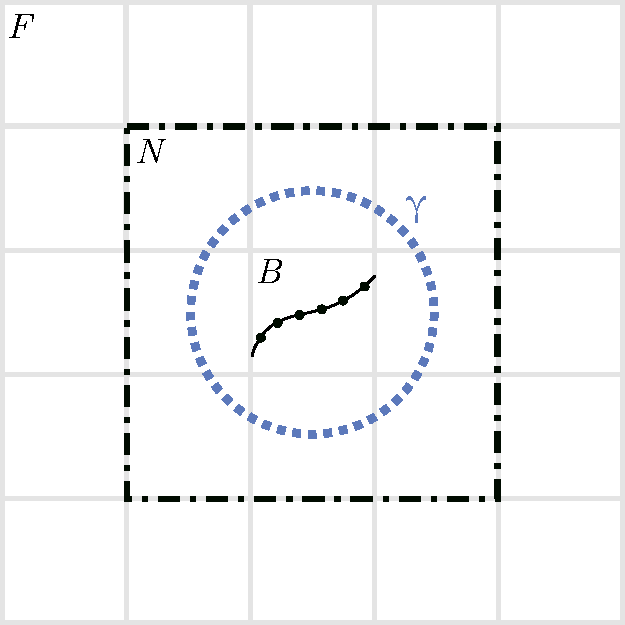
\includegraphics[width=0.5\textwidth]{ch_3/proxy.pdf}
    \caption{Considering the outgoing problem due to charge contained on $\Gamma \cap B$ evaluated in the far-field of $B$ in $\mathbb{R}^2$.}
    \label{fig:sec_3_1:proxy_trick}
\end{figure}

We can choose to represent our solution due to the charge in $B$ in $\mathcal{F}$ however we wish. However, our choice will lead to different matrices that we must compress.

Generally, we'll end up with a solution matrix of the form $A_{\mathcal{F}B}$ that maps between the charge contained $B$, $\psi_B$, and potential, $v_\mathcal{F}$, at points in its far-field that can be split up as,

\begin{flalign}
    v_{\mathcal{F}} &= A_{\mathcal{F}B} \psi_B \\
    &= B_{\mathcal{F}\gamma} C_{\gamma B} \psi_B
\end{flalign}

the subscripts indicate the domains these operators map between. We desire a split like this as the far field interaction of $B$ can be expressed as an object involving $C_{\gamma B}$ only.

To see how such a split can be useful consider the fact that $A_{\mathcal{F}B}$ can be written as,

\begin{flalign}
    \label{eq:decomposition}
    A_{\mathcal{F}B} = \begin{bmatrix}
        A_{\mathcal{Q}B}\\ A_{\mathcal{P}B}
        \end{bmatrix} = \begin{bmatrix}
        I & 0\\ 0 & B_{\mathcal{P}\gamma}
        \end{bmatrix} \begin{bmatrix}
        A_{\mathcal{Q}B}\\ C_{\gamma B}
        \end{bmatrix}
\end{flalign}

Our RS-S algorithm relies on a compression of this matrix, however as we noted a direct compression of $A_{\mathcal{F} B}$ is too expensive. However if we can find a decomposition like above, we can apply an interpolative decomposition to the right column in (\ref{eq:decomposition}) which has dimensions $O(1) \times O(n_\gamma)$ by construction where $n_\gamma$ is the number of proxy points. To prove that this allows us to reconstruct the full matrix after compression. Consider an ID that gives us,

\begin{flalign}
    \begin{bmatrix}
        A_{\mathcal{Q}B}\\ C_{\gamma B}
        \end{bmatrix} = \begin{bmatrix}
            A_{\mathcal{Q}S}\\ C_{\gamma S}
        \end{bmatrix} \begin{bmatrix}T_{SR}  & 1 \end{bmatrix}
\end{flalign}

Where $S$ and $R$ are the skeleton and redundant points respectively. Plugging back into our expression (\ref{eq:decomposition}),

\begin{flalign}
    \label{eq:compressed}
    A_{\mathcal{F}B} &=
        \begin{bmatrix}
            I & 0\\ 0 & B_{\mathcal{P}\gamma}
        \end{bmatrix}
        \begin{bmatrix}
             A_{\mathcal{Q}S}\\ C_{\gamma S}
        \end{bmatrix}
        \begin{bmatrix}T_{SR}  & 1 \end{bmatrix} \\
        &=\begin{bmatrix}
            A_{\mathcal{Q}S}\\ B_{\mathcal{P} \gamma}C_{\gamma S}
       \end{bmatrix} \begin{bmatrix}T_{SR}  & 1 \end{bmatrix} \\
       &=  A_{\mathcal{F}S} \begin{bmatrix}T_{SR}  & 1 \end{bmatrix}
\end{flalign}

Therefore, we see that we can get away with a cheap ID to reconstruct the far-field operator, involving the proxy points rather than the full far field of $B$. We are thus left with the task of formulating the proxy trick to compress the correct components of the boundary integral kernel.

Below we consider how to apply the proxy trick for different representations of the far-field potential due to the charges contained in $B$, known as `outgoing skeletonisations', as well the inverse operation in which the proxy trick is applied to calculate the potentials within $B$ due to charges in its far-field, known as `incoming skeletonisations'.

\subsubsection*{Hypersingular - $\mathcal{T}$}

\subsubsection*{Outgoing Skeletonisation}

A double-layer potential, due to some unknown density $\psi$, supported on $\tau$,

\begin{flalign}
    v(x) = \int_{\Gamma \cap B} \frac{\partial \Phi(x, y)}{\partial n(y)} \psi(y) ds(y) := \mathcal{D}\psi, \> \> x \in \mathbb{R}^m \setminus \tau
\end{flalign}

solves the Helmholtz equation everywhere it's valid. Here, $\Phi(x, y)$ is the fundamental solution of the Helmholtz equation. However, its normal derivative evaluated at the target points, known as the hypersingular operator, which we'll need for deriving boundary integral equations for Maxwell problems, does not,

\begin{flalign}
    \frac{\partial v}{\partial n(x)} = \frac{\partial}{\partial n(x)} \int_{\Gamma \cap B} \frac{\partial \Phi(x, y)}{\partial n(y)} \psi(y)ds(y) := \mathcal{T}\psi, \> \> x \in \Gamma \cap \mathcal{F}
\end{flalign}

it's only valid at far-field points, $\Gamma \cap \mathcal{F}$. However, we can separate out the normal part of the derivative,

\begin{flalign}
    \frac{\partial v}{\partial n(x)} = n(x) \cdot \nabla_x \int_{\Gamma \cap B} \frac{\partial \Phi(x, y)}{\partial n(y)} \psi(y)ds(y) := n \cdot w
\end{flalign}

The function

\begin{flalign}
    w(x) = \nabla_x \int_{\Gamma \cap B} \frac{\partial \Phi(x, y)}{\partial n(y)} \psi(y)ds(y) := \nabla_x \mathcal{D}\psi
\end{flalign}

Does satisfy our PDE, everywhere, and we'll exploit this fact in a moment. As an aside, we can see that this is true by considering a double layer potential $v$ that is smooth enough to admit,

\begin{flalign}
    (\Delta + k^2)w =(\Delta + k^2)\nabla_x v =\nabla_x (\Delta + k^2) v = 0
\end{flalign}

where the last equality follows as $v$ satisfies the Helmholtz equation. Therefore $w$ is a solution of the Helmholtz equation. Note that $w$ has three components.

In order to find our $C_{\gamma B}$ with this representation, we need to set up an `associated boundary value problem' for each component of $w$. The choice of boundary value problem we choose is free, as we only rely on the existence of its solution.

Consider an associated boundary value problem for just a single component of $\tilde{w}$ that satisfies,

\begin{flalign}
    &(\Delta + k^2)\tilde{w} = 0, \> \> x \in \mathbb{R}^m \setminus D \\
    &\tilde{w} = w_1(x) \\
    &\text{A radiation condition at } \infty
\end{flalign}

A combined field representation might be nice, as we know it has good properties,

\begin{flalign}
    \tilde{w} = (\mathcal{D} - ik \mathcal{S})_{\mathcal{F}\gamma} \mu
\end{flalign}

where $\mu$ is some unknown density supported on the proxy surface $\gamma$. Forming the boundary integral equation, and plugging back into the representation for $\tilde{w}$,

\begin{flalign}
    \tilde{w} &=  (\mathcal{D} - ik \mathcal{S})_{\mathcal{F} \gamma}(\frac{1}{2}\mathcal{I} + \mathcal{D} - ik \mathcal{S})_{\gamma \gamma}^{-1}w_1 \\
    &= (\mathcal{D} - ik \mathcal{S})_{\mathcal{F} \gamma}(\frac{1}{2}\mathcal{I} + \mathcal{D} - ik \mathcal{S})_{\gamma \gamma}^{-1} \nabla_1 \mathcal{D}_{\gamma B} \psi_\gamma \\
    &\equiv B_{\mathcal{F}\gamma} C_{\gamma B} \psi_\gamma
\end{flalign}

where we identify,

\begin{flalign}
    C_{\gamma B} = \nabla_1 \mathcal{D}_{\gamma B}
\end{flalign}

This is the matrix we will attempt to compress. Similar analysis follows for the other two components of $w(x)$. Meaning that we end up having to compress $[\nabla_1 \mathcal{D}_{\gamma B} , \nabla_2 \mathcal{D}_{\gamma B} , \nabla_3 \mathcal{D}_{\gamma B}]$ for the outgoing problem. We note that $B_{\mathcal{F} \gamma }$ is never explicitly formed, we just require its existence. When we calculate an approximation of $A_{\mathcal{F}B}$ using (\ref{eq:compressed}), we only need to know the ID of the $C_{\gamma B}$.

\subsubsection*{Incoming Skeletonisation}

For the incoming skeletonization, were again we're considering the same representation with a hypersingular operator, we observe that we're just looking for,

\begin{flalign}
    \left [\frac{\partial v}{\partial n(x)} \right ]_{\mathcal{F} B}^T
\end{flalign}

with the formation of an associated boundary integral equation taking place in much the same way as for the outgoing problem. However, the hypersingular operator is self-adjoint, therefore it leads to the same expressions for $C_{\gamma B}$.

\subsubsection*{Derivative of the Single Layer - $\mathcal{K}'$}

\subsubsection*{Outgoing Skeletonisation}

If we choose to represent our potential with a single-layer potential,

\begin{flalign}
    u(x) = \int_{\Gamma \cap B} \Phi(x, y) \phi(y) ds(y) := \mathcal{S}\phi, \> \> x \in \mathbb{R}^m \setminus \tau
\end{flalign}

and seek a boundary integral equation in terms of its normal derivative at the targets,

\begin{flalign}
    w(x) = \int_{\Gamma \cap B} \frac{\partial \Phi(x, y)}{\partial n(x)} \phi(y) ds(y) := \mathcal{K}'\phi, \> \> x \in \Gamma \cap \mathcal{F}
\end{flalign}

We observe the same problem as in the $\mathcal{T}$ case, where this expression is not a general solution of our PDE. We can similarly separate out the normal component and write,

\begin{flalign}
    \tilde{w}(x) := \int_{\Gamma \cap B} \nabla_x \Phi(x, y) \phi(y) ds(y), \> \> x \in \mathbb{R}^m \setminus \tau
\end{flalign}

Using the previous analysis for $\mathcal{T}$, we immediately recognise that the components we must compress are $C_{\gamma B} = \nabla_1 \mathcal{S}_{\gamma B}$, giving us $[\nabla_1 \mathcal{S}_{\gamma B}, \nabla_2 \mathcal{S}_{\gamma B}, \nabla_3 \mathcal{S}_{\gamma B}]$ to compress in total for the outgoing problem.

\subsubsection*{Incoming Skeletonisation}

Noticing that,

\begin{flalign}
    \left [\frac{\partial u}{\partial n(x)} \right ]_{\mathcal{F} B}^T = \int_{\Gamma \cap B} \frac{\partial \Phi(x, y)}{\partial n(y)} \phi(y) ds(y) = \mathcal{D}_{\gamma B} \phi
\end{flalign}

already satisfies our PDE without any further work, we can simply use it as our Dirichlet data in the associated boundary value problem. The matrix to compress being $C_{\gamma B} = \mathcal{D}_{\gamma B}$.

\subsubsection*{Single Layer - $\mathcal{S}$}

\subsubsection*{Outgoing Skeletonisation}

We now choose to represent our scattered solution with a single-layer operator,

\begin{flalign}
    u(x) =\int_{\Gamma \cap B} \Phi(x, y)\phi(y)ds(y) := \mathcal{S}\phi,\> \> x \in \mathbb{R}^m \setminus \tau
\end{flalign}

This satisfies the underlying PDE everywhere. We can now set up an associated exterior boundary value problem as before, and use our single-layer potential as Dirichlet boundary data.

\begin{flalign}
    (\Delta + k^2)w= 0, \> \> x \in \mathbb{R}^m \setminus D \\
    w = \mathcal{S}\phi, \> \> \text{on } \gamma \\
    \text{Radiation condition at }\infty
\end{flalign}

where $\phi$ is some unknown density supported on $\tau$. As before, we can form a boundary integral equation for this associated problem, and solve, recognising that the matrix to compress $C_{\gamma B} = \mathcal{S}_{\gamma B}$

\subsubsection*{Incoming Skeletonisation}

The single-layer operator is self-adjoint, leading to the same operator to compress. Spelling this out, consider the associated interior boundary value problem,

\begin{flalign}
    (\Delta + k^2)w= 0\> \> \text{in } D \\
    w = \mathcal{S}\phi \> \> \text{on } \gamma
\end{flalign}

The solution of an interior Helmholtz scattering problem may not be unique, but this doesn't matter for our purposes. Proxy compression doesn't require uniqueness, only existence. Let's seek a solution in the form of a combined-layer potential,

\begin{flalign}
    w(x) = (\mathcal{D}_\gamma - ik \mathcal{S}_\gamma)[\phi](x)
\end{flalign}

where the subscripts make it clear that the density is supported on $\gamma$. Forming the boundary integral equation,

\begin{flalign}
    (-\frac{\mathcal{I}}{2} + \mathcal{D}_\gamma - ik \mathcal{S}_\gamma)[\phi](x) = \mathcal{S}_{\mathcal{F} \gamma}[\phi](x)
\end{flalign}

Solving with the representation gives,

\begin{flalign}
    w = \mathcal{S}_{B \gamma}(-\frac{\mathcal{I}}{2} + \mathcal{D}_\gamma - ik \mathcal{S}_\gamma)^{-1}\mathcal{S}_{\gamma \mathcal{F}}[\phi](x) = C_{B \gamma}B_{\gamma \mathcal{F}}
\end{flalign}

where we recognize the matrix to compress as $C_{B\gamma} = \mathcal{S}_{B\gamma}$ in our proxy framework.

\subsection*{Double Layer - $\mathcal{D}$}

\subsubsection*{Outgoing Skeletonisation}

A double-layer potential, due to some unknown density $\psi$, supported on $\tau$,

\begin{flalign}
    v(x) = \int_{\Gamma \cap B} \frac{\partial \Phi(x, y)}{\partial n(y)} \psi(y) ds(y) := \mathcal{D}\psi, \> \> x \in \mathbb{R}^m \setminus \tau
\end{flalign}

solves the Helmholtz equation everywhere it's valid. Therefore it can be used as Dirichlet data for the associated boundary value problem for the outgoing skeletonization. Applying similar analysis to above, we identify the kernel to compress as $C_{\gamma B} = \mathcal{D}_{\gamma B}$.

\subsubsection*{Incoming Skeletonisation}

We notice that the transpose of the double layer operator is,

\begin{flalign}
    [u]^T_{\mathcal{F}B}(x) = \int_{\Gamma \cap B} \frac{\partial \Phi(x,y)}{\partial n(x)}\phi(y)ds(y)= \mathcal{K}'_{\gamma B}\phi
\end{flalign}

This in general does not satisfy our PDE everywhere, we again separate out the normal component, and as before, recognise that the components to compress are $[\nabla_1 \mathcal{S}_{\gamma B}, \nabla_2 \mathcal{S}_{\gamma B}, \nabla_2 \mathcal{S}_{\gamma B}]$.

\subsection*{Acoustic Sound Hard Scattering}

Let's now apply our fast direct solver framework, with proxy compression to some example problems. We begin with acoustic sound-hard scattering, which is a didactic example. Consider a scattered field $u^s$, that scatters off an object $\Omega$ and satisfies the Helmholtz equation in the exterior,

\begin{flalign}
    (\Delta + k^2)u^s = 0, \> \> \> \text{in  } \mathbb{R}^3 \setminus \Omega
\end{flalign}

The `sound hard' boundary condition on the surfae $\Gamma$ is
\begin{flalign}
    \frac{\partial u^s}{\partial n} = \frac{\partial u^{i}}{\partial n}, \> \> \> \text{in  } \Gamma
\end{flalign}

where $u^i$ is the incident wave. Using the analysis in \cite{Bruno2012}, we write down a `regularised' representation formula for our solution. This regularisation can be shown to have better spectral properties.

\begin{flalign}
    u^s =(\mathcal{K}_k \circ \mathcal{S}_K - i\eta \mathcal{S}_k)
\end{flalign}

where $k$ and $K$ are complex wave numbers, that may not be the same. We can take the trace of this representation, and its normal derivative at the targets, and find a boundary integral equation for the exterior problem,

\begin{flalign}
    (\frac{i \eta}{2} \mathcal{I}- i \eta \mathcal{K}'_k + \mathcal{T}_k \circ \mathcal{S}_K )\mu = g
\end{flalign}

using the Calder\'{o}n identity,

\begin{flalign}
    \mathcal{T}_k\circ \mathcal{S}_k = -\frac{1}{4}\mathcal{I} + \mathcal({K}_k')^2
\end{flalign}

which is true for any $k$, we arrive at a boundary integral equation,

\begin{flalign}
    \left ( i \eta(\frac{1}{2}\mathcal{I}  - \mathcal{K}'_k) - \frac{1}{4}I+ \mathcal({K}_k')^2 \right ) \mu = g
\end{flalign}

by defining $\theta := \mathcal{K}'_k \mu$, we can write the boundary integral equation as a system,

\begin{flalign}
\begin{pmatrix}
(\frac{i\eta}{2} - \frac{1}{4})\mathcal{I} - i \eta \mathcal{K}'_k & \mathcal{K}'_k  \\
 \mathcal{K}'_k & - \mathcal{I}
\end{pmatrix}
\begin{pmatrix} \mu \\ \theta \end{pmatrix} = \begin{pmatrix}
    g \\ 0
\end{pmatrix}
\end{flalign}

We can then place this system into our fast direct solver framework. Despite not knowing how to compress the system matrix altogether, we do know how to compress each block, as they each correspond to displacements of $\mathcal{K}'_k$.

Consider writing out our block matrix as,


\begin{flalign}
    \begin{pmatrix}
        A & B \\ C & D
    \end{pmatrix}
    \begin{pmatrix}
        \mu\\\theta
    \end{pmatrix}
   = \begin{pmatrix}
        g\\ 0
    \end{pmatrix}
\end{flalign}

and re-writing as,

\begin{flalign}
    \begin{pmatrix}
        \begin{pmatrix}
            A_{11} & B_{11} \\ C_{11} & D_{11}
        \end{pmatrix} & . & .\\
        . & . & \\
        . & &     \begin{pmatrix}
            A_{NN} & B_{NN} \\ C_{NN} & D_{NN}
        \end{pmatrix}
    \end{pmatrix}
    \begin{pmatrix}
        \mu_1 \\ \theta_1 \\ . \\ . \\ \mu_n \\ \theta_n
    \end{pmatrix} =
    \begin{pmatrix}
        g_1 \\ 0 \\ . \\ . \\ g_N \\ 0
    \end{pmatrix}
\end{flalign}

This system matrix remains numerically low-rank, and therefore can fit into our RS-S framework. Indeed, we now have to compress a system of matrix operators in order to capture its row space via the proxy trick.

\subsection*{Preliminary Numerical Experiments}

The paper on which we base our work \cite{sushnikova2022fmm} builds on the original RS-S algorithm \cite{minden2017recursive} by:

\begin{enumerate}
    \item Implementing generalized Gaussian quadratures for computing near-field interactions \cite{bremer2013numerical}.
    \item Determining a properly sampled discretisation of the proxy surface which depends on the box size in the octree, so as to sufficiently sample oscillatory kernels without oversampling.
    \item Handling the construction of the far-field partition into $\mathcal{F} = \mathcal{Q} \cup \mathcal{P}$
\end{enumerate}

We defer to to the original paper for a discussion of these aspects \cite{sushnikova2022fmm}. For our simulations we use these algorithms and quadrature rules as a black box in as implemented by the FMM3D-BIE software \cite{fmm3dbie}. To demonstrate the accuracy of the solver in light of our proxy trick formulation, we suppose that the sound hard condition is generated from a set of 50 test points placed at random locations on the surface of a test geometry, for which we choose the `wiggly torus' displayed in figure (\ref{fig:octree_example:sec_1_2}). The results of our solve are then compared to the potential expected from using a combined field representation at 50 random test locations in the exterior of the geometry.

\begin{flalign*}
    \text{error} = \frac{\sqrt{\sum_{j=1}^{50}|\tilde{u}(t_j)-u(t_j)|^2}}{\sqrt{\int_\Gamma|\sigma(x)|^2 da(x)}}
\end{flalign*}

where $\tilde{u}$ is our approximated potential, $u$ is the exact potential calculated from our test points, $t_j$, and $\sigma$ is the calculated charge density from the boundary integral equation. The torus is taken to be in a bounding box, each dimension of which is fixed at $1 \lambda$ where $\lambda$ is the wavelength of the incident wave, and we fix the error of the ID at $\epsilon = 5 \times 10^{-7}$, and the wavenumber $k=0.97$. Experiments are taken on a single-node of the Rusty Cluster at the Flatiron Institute, which consists of 240 28-core Intel Broadwell nodes with 512GB of RAM.

\begin{table}[h!]
    \centering
    \begin{tabular}{||c c c c c c c c||} 
        \hline
        $p$ & $N_{patch}$ & $N$  & $t_f$ (s) & $t_s$ (s)  & $t_q$ (s) & $m_f$ (GB) & $\epsilon$ \\ [0.5ex]
        \hline\hline
        4 & 50  & 750  & 0.8 & 0.03 & 0.8 & 0.04 & $4.7 \times 10^{-3}$ \\
        4 & 200 & 3000 & 6.6 & 0.08 & 1.4 & 0.6  & $3.3 \times 10^{-4}$ \\
        4 & 450 & 6750 & 84.9 & 0.2 & 2.5 & 2.9 & $5.2 \times 10^{-5}$ \\
        4 & 800 & 12000 & 324.9 & 0.6 & 4.2 & 7.5 & $1.6 \times 10^{-5}$ \\
        4 & 1250 & 18750 & 1138.8 & 1.1 & 6.2 & 15.2 & $5.8 \times 10^{-6}$ \\
        4 & 1800 & 27000 & 1839.7 & 1.7 & 8.8 & 25.2 & $2.4 \times 10^{-6}$ \\
        4 & 2450 & 36750 & 3322.6 & 2.4 & 11.8 & 41.1 & $1.2 \times 10^{-6}$ \\
        \hline
    \end{tabular}
    \caption{We measure the $L^2$ error with respect to the density  ($\epsilon$), time for solution ($t_s$), factorisation ($t_f$), quadrature computation ($t_q$) and memory required for factorisation ($m_f$) as a function of quadrature expansion order ($p$) and number of patches used to discretise the geometry ($N_{patch}$).}
    \label{table:sec_3_2:sh}
\end{table}


From table (\ref{table:sec_3_2:sh}), we observe linear scaling for $t_f$. However we observe sub-linear scaling for for $m_f$ and $t_s$, the authors of \cite{sushnikova2022fmm} suggest that this is due to the fixed wavenumber for increasing $N$. Meaning that the additional degrees of freedom introduced beyond a certain sampling in points per wavelength are more easily compressed. In order to make further observations about the convergence rate of our method more data is required, for higher order quadratures. We note that amount of memory used, even for the modest problem sizes tested, can be quite considerable. With our experiment where the number of quadrature points $N=36750$ consuming over 40GB of memory. This demonstrates the main trade-off of fast direct solvers in comparisons to iterative solvers.

\subsection*{Exposing Parallelism}

The RS-S algorithm exposes natural parallelism. Consider figure (\ref{fig:sec_3_1:rss_parallel}) which shows a four-colouring for a non-adaptive octree in $\mathbb{R}^2$ for simplicity, each colour can be independently skeletonised as skeletonisation only updates matrix entries corresponding to a box's near field. The same logic can be applied to the adaptive case, as well as the $\mathbb{R}^3$ case, albeit with more colours. As of writing there are no parallel implementations of the RS-S algorithms available as open-source packages.

\begin{figure}
    \centering
    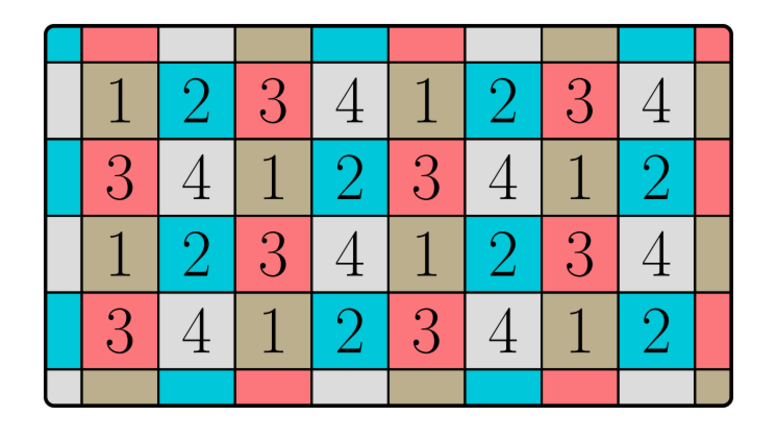
\includegraphics[width=0.5\textwidth]{ch_3/rss-parallel.pdf}
    \caption{A four-colouring of a non-adaptive quadtree in $\mathbb{R}^2$, where the colouring is chosen such that no box shares a colour with its neighbours. All boxes of a given colour can then be skeletonised independently. This figure is adapted from \cite{minden2017recursive}.}
    \label{fig:sec_3_1:rss_parallel}
\end{figure}